%% wp0 引言与动机（论文第 1 节）
\wph{引言与动机}

现代 GPU 越来越多地针对以张量（tensor）为中心的计算进行优化，其驱动力来自深度学习与科学计算的需求。NVIDIA 的 Volta 架构（NVIDIA，2017）引入了 Tensor Core，使硬件能够直接高效地完成小矩阵乘法。这一能力在 Turing（NVIDIA，2018）与 Ampere（NVIDIA，2021）中得到扩展，提供了在 GPU 内存层次结构中进行结构化矩阵搬运的专用指令。Hopper（NVIDIA，2023）与 Blackwell（NVIDIA，2025）架构进一步推进了这一范式，引入了在全球内存与共享内存之间高效传输 5 阶（rank）张量的拷贝指令，并进一步扩展了 Tensor Core 的能力。GPU 峰值性能很大程度上取决于这些面向张量的硬件特性能否被充分发挥，能高效表示与操作这些张量的高性能编程模型也就应运而生。

现有及新兴的硬件表现如何，很大程度上取决于多维数据在多个层次化内存空间与多个层次化并行级别中怎样被存储与访问。数据存储布局（layout）历来通过决定内存访问发生的方式与时机来影响性能；而随着硬件指令的规模越来越大，并为其输入输出规定了固定的布局，布局也开始决定正确性。这些布局必须沿整条执行流水线传递下去，才能保证硬件指令被正确调用，并保证内存访问模式得到优化。

在本工作中，我们呈现 \CuTe 的基础概念。\CuTe 是一项针对 \underline{CU}DA \underline{Te}nsors（即 \underline{C}ompute \underline{U}nified \underline{Te}nsors）的规约，旨在为编写峰值性能的线性代数库提供建构基石。\CuTe 的核心是两项关键创新：
\begin{compactitem}
\item {\em 一种新颖的张量布局表示}：\CuTe 的形状（shape）、布局与张量天然是层次化的，由更小的嵌套实例构造而成。这种层次结构提供了表示现代张量指令所需复杂映射的手段，同时仍是 {\tt BLAS}、{\tt torch.tensor}、{\tt numpy.ndarray} 与 MATLAB 等库中既有的扁平形状与扁平步幅（stride）表示的严格扩展。
\item {\em 一种定义在布局之上的新颖操作代数}：\CuTe 布局支持一组丰富的操作，包括拼接（concatenation）、合并（coalescence）、复合（composition）、补（complementation）、切分（division）、分块（tiling）与求逆（inversion），它们的结果都仍是新的 \CuTe 布局。这些操作支撑现代张量指令所需的复杂划分（partitioning）、操纵、验证与推导。
\end{compactitem}

\CuTe 的布局表示给通用算法一个直观的框架来管理线程与数据，布局代数则给高性能线性代数 kernel 的开发一条有表达力的路径，用来操纵布局、生成新布局。两者能带来：
\begin{compactitem}
\item 对复杂布局与划分的支持：\CuTe 便于表示应用特定数据模式所需的精细布局，以及专用张量指令所需的复杂划分模式。
\item 关注点分离：数据布局独立于算法逻辑进行声明，提升清晰性与模块化。
\item 静态分析与优化：精深的代数技术使我们能够依据体系结构约束对张量参数进行检查、重排与划分。
\end{compactitem}

\wpsh{相关工作}

\CuTe 的动机源于支持高效张量收缩开发的需求：张量收缩是众多科学计算与机器学习应用的核心。计算一般张量收缩的传统方法依赖矩阵化，即在逻辑上或显式地重组张量数据，以便通过一系列对基础线性代数子程序（BLAS）库的调用来完成计算。

%鉴于大多数张量收缩的理论计算与通信复杂度与矩阵乘法等价，张量收缩运算原则上能够以相似的效率扩展。

BLAS 为核心线性代数运算提供了高效且可移植的实现，并为广泛的体系结构提供了高度优化的版本（Blackford 等，2002）。在 BLAS 原语中，通用矩阵乘法（GEMM）例程无疑是全部科学计算与机器学习中被优化得最充分、使用最广泛的操作。

类 BLAS 库实例化软件（BLIS）框架（Van Zee 与 van de Geijn，2015）扩展了 GEMM，使其同时支持行模与列模中的非单位步幅，从而在不借助显式内存拷贝的情况下解决了处理不规则内存布局的部分挑战。BLAS 的跨步批量（strided-batched）GEMM 扩展进一步推广了该原语，使其能够应用于更多张量收缩（Shi 等，2016）。在对矩阵布局做更进一步的抽象时，启发 \CuTe 的思路是：在张量记号中使用多重索引，使任意张量收缩都能变换为规范化的 batched-GEMM 原语。

许多现有库都依赖张量，而它们几乎全都基于扁平形状与扁平步幅表示。在 Python 中，这包括 {\tt numpy.ndarray} 与 {\tt torch.tensor}：

\noindent
\begin{minipage}[t]{0.48\textwidth}
\begin{python}
>>> import numpy
>>> a = numpy.ndarray([3,7,5])
>>> a.dtype
dtype('float64')
>>> a.shape
(3, 7, 5)
>>> a.strides
(280, 40, 8)
\end{python}
\end{minipage}
\hfill
\begin{minipage}[t]{0.48\textwidth}
\begin{python}
>>> import torch
>>> a = torch.empty(3,7,5)
>>> a.dtype
torch.float32
>>> a.shape
torch.Size([3, 7, 5])
>>> a.stride()
(35, 5, 1)
\end{python}
\end{minipage}

\noindent 在 C++ 中，则是 {\tt std::mdspan}：

\noindent
\begin{cpp}
std::mdspan a = std::mdspan(data, 3, 7, 5);
a.extent(0);  // 3
a.extent(1);  // 7
a.extent(2);  // 5
a.stride(0);  // 35
a.stride(1);  // 5
a.stride(2);  // 1
\end{cpp}

\noindent \CuTe 支持这些表示，并对其做严格扩展：推广到层次化的形状与步幅，以表示更复杂的布局、非整数步幅以及非整数的布局陪域。

对稠密张量表示的独立推广还包括 HeLayers（Aharoni 等，2023）、ThunderKittens（Spector 等，2024），以及 OpenAI 的 Triton 编译器（Tillet 等，2019）中所使用的 Linear Layouts（Zhou 等，2025）方法。ThunderKittens 为寄存器内存、共享内存、行主序/列主序块、由行主序/列主序子块组成的行主序/列主序块，以及为 warp 与线程规定的访问模式实现了种类繁多的定制类型。这些类型的编写考虑了体系结构布局需求与内存层次，但其表示范围局限于既有的类型与模式。Linear Layouts 基于 $\mathbb{F}_2$ 线性代数，为张量布局提供了更一般的表示，也为布局分析与生成开辟了途径。但 Linear Layouts 对 $\mathbb{F}_2$ 的严格依赖使其中一些算子难以被人工检视，并将该工作限制在 2 的幂形状与步幅上，这对许多应用来说是不可接受的。

另一些启发了本工作部分内容的布局分析方法同样依赖 $\mathbb{F}_2$ 线性代数，例如 Edelman 等（1994）、Cormen（1993）与 Bouverot-Dupuis 及 Sheeran（2023）的工作。这些工作给出了分析与算法生成的出发点，但受限于其撰写时的应用语境。

由于 CUTLASS v3（NVIDIA，2023）中 \CuTe 的 C++ 实现是开源的并附有部分文档，它已在分析 \CuTe 布局与 \CuTe 代数操作的独立工作中被引用和使用。Bhaskaracharya 等（2025）在整数集关系（ISL）的语境下分析了 \CuTe 与 Linear Layouts（Zhou 等，2025），但略去了能将 Linear Layouts 表示为 \CuTe 布局的步幅抽象。LEGO（Tavakkoli 等，2025）在代码生成器中使用受限形式的 \CuTe 布局与原始形式的 \CuTe 复合来生成复杂索引。Carlisle 等（2026）则在范畴论的语境下分析了 \CuTe 布局及作用于其上的若干操作。
在本文中，我们打算对 \CuTe 概念及其应用给出更明确、更形式化的论述，并提供 \CuTe 的一个 Python 参考实现。
纯 Python 的参考实现 PyCuTe（NVIDIA，2026）可在 \url{https://github.com/NVlabs/CuTe} 获取，它与本文的定义与后置条件一一对应；它不同于面向 CUDA kernel JIT 编译的 CuTe DSL（NVIDIA，2025），也不同于 CUTLASS 中的 C++ CuTe 头文件。

\CuTe 的设计与概念已在若干应用中落地。例如，Graphene 张量编译器（Hagedorn 等，2023）用 \CuTe 表示张量运算；Stream-K 算法（Osama 等，2023）的实现用了 \CuTe 的 C++ 实现，NVIDIA CUTLASS v3 库（Kerr 等，2017）的开发也以它为核心。大型语言模型最先进的实现中也一直有它，FlashAttention 及其一代代演进（Dao 等，2022、Dao，2023、Shah 等，2024）就是例子，深度学习前沿的研究与应用处处用得上 \CuTe。一批相关编译器项目同样建在 \CuTe 之上，包括 CuTe DSL（NVIDIA，2025）：一种面向线性代数应用、基于 Python、动态编译 CUDA 软件的 DSL。

\wpsh{规范化循环与循环变换}
\label{sec:loops}

循环索引的显式计算是高性能线性代数 kernel 开发中的常见挑战。这些计算很难被程序员一次写对，维护起来更是难上加难。与其将数据访问信息与算法逻辑耦合在一起，我们更愿意用矩阵/向量坐标（coordinate）清晰地书写算法逻辑，而将数据访问模式抽象到数据布局之中。

为便于说明，我们首先定义本工作所发展的技术能够处理的循环嵌套类别。具体而言，我们把{\em 标准循环形式}（standard loop form）定义为具有单个索引、从零开始、以常量为界、且每次迭代递增 1 的循环。

例如，考虑如下循环：
\begin{cpp}
for (int m = 2; m <= 50; m += 3)
  A[m] = e(m);
\end{cpp}
该循环将 {\tt A[2]}、{\tt A[5]}、{\tt A[8]}、$\ldots$ 设为纯表达式 {\tt e(m)} 的结果。它可以变换为如下的规范化循环（canonical loop）：
\begin{cpp}
for (int i = 0; i < 17; ++i)
  (A + 2)[3*i] = g(i);
\end{cpp}
这里，指针偏移了一个循环不变常量，循环步幅被归一化为 1，下界变换为零，上界紧致且不含端点，纯表达式变换为 {\tt g(i) = e(3*i+2)}。现在，把上例理解为遍历一个逻辑上的 17 元素向量是很自然的：逻辑坐标以 3 为步幅，对基地址 {\tt A + 2} 处的数据进行索引。该程序可用如下数据表示：
\begin{verbatim}
Accessor: A + 2
   Shape: 17
  Stride: 3
\end{verbatim}
嵌套循环可以类似地处理。考虑如下的二维循环嵌套：
\begin{cpp}
for (int n = 3; n < 43; n += 2)
  for (int m = 4; m <= 22; m += 5)
    A[p*m + q*n] = e(m,n);
\end{cpp}
它可以变换为规范化循环形式：
\begin{cpp}
for (int j = 0; j < 20; ++j)
  for (int i = 0; i < 4; ++i)
    (A + 4*p + 3*q)[5*p*i + 2*q*j] = g(i,j);
\end{cpp}
有了规范化循环嵌套，很自然地可以把变换后的循环理解为遍历一个逻辑上的 $4 {\times} 20$ 矩阵：逻辑行坐标 $i$ 以 $5p$ 为步幅，逻辑列坐标 $j$ 以 $2q$ 为步幅，对基地址 {\tt A + 4*p + 3*q} 处的数据进行索引。这可以用如下数据表示：
\begin{verbatim}
Accessor: A + 4p + 3q
   Shape: ( 4, 20)
  Stride: (5p, 2q)
\end{verbatim}
一个关键观察是，$4 {\times} 20$ 矩阵也可以被解释为一个具有非均匀、半仿射步幅的 80 元素向量，用等价的规范化循环形式表达即为：
\begin{cpp}
for (int k = 0; k < 80; ++k)
  (A + 4*p + 3*q)[5*p*(k%4) + 2*q*(k/4)] = f(k);
\end{cpp}
其中 {\tt \%} 是取模运算，{\tt /} 是整数向下取整除法。这一变换是 2 维坐标 \verb|(i,j)| 与 1 维坐标 \verb|k| 之间的余字典序（colexicographical）双射 \verb|(i,j) = (k%4,k/4)|。
该双射与先前表示的形状等价，并可由其直接推导而来。因此，该形状表示既可以接受 2 维坐标，也可以接受 1 维坐标，为数据索引提供了一个灵活且与阶无关的框架。

规范化循环形式还为可证正确的循环变换提供了指导，这类变换经常出现在面向张量计算的优化编译器中。考虑最一般的规范化循环嵌套：
\begin{cpp}
for (int in = 0; in < Nn; ++in)
  ...
    for (int i1 = 0; i1 < N1; ++i1)
      for (int i0 = 0; i0 < N0; ++i0)
        A[d0*i0 + d1*i1 + ... + dn*in] = e(i0,i1,...,in);
\end{cpp}
其中 $(N_0, N_1, \ldots, N_n)$ 是计算的“形状”，$(d_0, d_1, \ldots, d_n)$ 是访问模式的“步幅”，
\begin{verbatim}
Accessor: A
   Shape: (N0,N1,...,Nn)
  Stride: (d0,d1,...,dn)
\end{verbatim}
由于 $\text{形状}:\text{步幅}$ 信息与循环嵌套本身之间存在一一对应，我们不必问“如何对循环施加变换——切分、转置、拼接、置换、截断、向量化等”，而是可以转而问：“$\text{形状}:\text{步幅}$ 表示的合法变换方式有哪些，又有哪些算子能提供这些变换？”事实上，若 $\v{L} = \text{形状}:\text{步幅}$ 表示数据访问与循环嵌套，那么存在哪些函数 $P$，使得
\begin{align*}
\v{L}' = P(\v{L}) = \v{L} \circ P
\end{align*}
构成从 $\v{L} = \text{形状}:\text{步幅}$ 到新循环嵌套 $\v{L}' = \text{形状}':\text{步幅}'$（可能具有新的形状与步幅）的一个有意义的变换？这些变换 $P$ 本质上是对循环嵌套的{\em 重写}，若定义得当，它们自身可以可复合、可求逆，并为命令式循环提供类似函数式编程的控制。结合上文讨论的 1 维坐标与 N 维坐标之间的双射，本文将证明：这些变换的一种非常有效的表示是 $P = \v{P} = \text{形状}^*:\text{步幅}^*$，正是我们用来表示数据访问与循环嵌套自身的同一类对象。

\wpsh{张量与折叠}

为了进一步阐述除 1 维坐标之外还能以 N 维坐标索引的形状这一动机，我们推广 Shi 等（2016）中将张量收缩映射到规范化类 BLAS 原语的观察。

在本工作中，张量用粗体字母表示，索引用小写字母表示，索引的界用对应的大写字母表示。张量的阶指它所拥有的维度（也称为模（mode））的数量。例如：
\begin{compactitem}
\item 标量 $\alpha$ 是 0 阶张量。
\item 向量 $\mathbf{a}_i$ 是 1 阶张量，其中 $0 \leq i < I$。
\item 矩阵 $\mathbf{A}_{mn}$ 是 2 阶张量，其中 $0 \leq m < M$ 且 $0 \leq n < N$。
\item 三路数组 $\mathbf{A}_{mnp}$ 是 3 阶张量，其中 $0 \leq m < M$、$0 \leq n < N$ 且 $0 \leq p < P$。
\end{compactitem}
对仅在等式单侧出现的重复索引隐含求和（爱因斯坦记号），因此张量收缩的一个实例是
\begin{align}
\v{C}_{stqp} = \v{A}_{stupr} \, \v{B}_{qtru},
\label{eqn:contraction}
\end{align}
它表示一个 5 阶张量与一个 4 阶张量收缩生成一个 4 阶张量。这类收缩在 {\tt numpy.einsum} 与 {\tt torch.einsum} 等接口中有紧凑的表达。

上面的张量收缩可以重写为
\begin{align*}
\v{C}_{(sp)(q)(t)} = \v{A}_{(sp)(ur)(t)} \, \v{B}_{(q)(ur)(t)},
\end{align*}
其中原张量收缩的各模被归为四类：
\begin{compactitem}
\item 行模（row modes）$\hat{m}$：出现在 $\v{A}$ 与 $\v{C}$ 中，而不出现在 $\v{B}$ 中。
\item 列模 $\hat{n}$：出现在 $\v{B}$ 与 $\v{C}$ 中，而不出现在 $\v{A}$ 中。
\item 归约模 $\hat{k}$：出现在 $\v{A}$ 与 $\v{B}$ 中，而不出现在 $\v{C}$ 中。
\item 批模 $\hat{\ell}$：出现在 $\v{A}$、$\v{B}$ 与 $\v{C}$ 中。
\end{compactitem}
这被称为张量{\em 折叠}（folding）。折叠一个张量并不需要任何显式拷贝，可以只是数据视图的变更。

作为张量折叠的一个显式例子，考虑图~\ref{fig:folding} 第一行所示的 8 元素 $2 {\times} 2 {\times} 2$ 张量。扁平表示为张量的每个模保存一个形状与一个步幅，用以索引物理数据。这种扁平表示与 C++ 的 {\tt std::mdspan}、PyTorch 的 {\tt torch.tensor}、NumPy 的 {\tt numpy.ndarray} 以及许多其它类似库所采用的表示完全相同。如第二行所示，通过将第三个模折叠进第一个模，该 $2 {\times} 2 {\times} 2$ 张量可以折叠成 $4 {\times} 2$ 矩阵。其结果可用形状为 $(4,2)$、步幅为 $(2,1)$ 的扁平表示。原则上，通过将第三个模折叠进第二个模，该 $2 {\times} 2 {\times} 2$ 张量也可以折叠成 $2 {\times} 4$ 矩阵。然而其结果不再具有扁平表示：不存在能表示第二个模的步幅的整数。

\begin{figure}[ht]
\centering
\scalebox{0.6}{
\begin{tikzpicture}[x={(0cm,-1cm)},y={(1cm,0cm)},every node/.style={minimum size=1cm, outer sep=0pt}]
\node[fill={rgb,255:red,175;green,175;blue,255}] at (0,0) {\Large a\strut};
\node[fill={rgb,255:red,175;green,175;blue,255}] at (0,1) {\Large b\strut};
\node[fill={rgb,255:red,175;green,255;blue,175}] at (0,2) {\Large c\strut};
\node[fill={rgb,255:red,175;green,255;blue,175}] at (0,3) {\Large d\strut};
\node[fill={rgb,255:red,255;green,255;blue,175}] at (0,4) {\Large e\strut};
\node[fill={rgb,255:red,255;green,255;blue,175}] at (0,5) {\Large f\strut};
\node[fill={rgb,255:red,255;green,175;blue,175}] at (0,6) {\Large g\strut};
\node[fill={rgb,255:red,255;green,175;blue,175}] at (0,7) {\Large h\strut};
\draw[color=black,thick,shift={(-0.5,-0.5)}] (0,0) grid (1,8);
\node at (-1,0) {\Large{\texttt{0}}};
\node at (-1,1) {\Large{\texttt{1}}};
\node at (-1,2) {\Large{\texttt{2}}};
\node at (-1,3) {\Large{\texttt{3}}};
\node at (-1,4) {\Large{\texttt{4}}};
\node at (-1,5) {\Large{\texttt{5}}};
\node at (-1,6) {\Large{\texttt{6}}};
\node at (-1,7) {\Large{\texttt{7}}};
\node at (1,3.5) {\Large 物理数据};
\end{tikzpicture}
}\\
\vspace{1em}
\begin{tabular}{|c|c|c|c|}
视图描述 & 视图图示 & 扁平表示 & \CuTe 表示 \\
\hline\hline
\shortstack{张量，$2 {\times} 2 {\times} 2$ \\ 3 阶} &
\scalebox{0.4}{
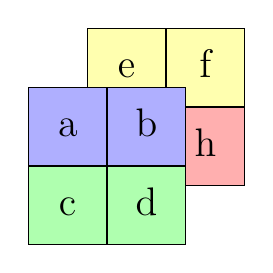
\begin{tikzpicture}[x={(0cm,-1cm)},y={(1cm,0cm)},every node/.style={minimum size=1cm, outer sep=0pt},baseline=(current bounding box.center)]
\node[draw=black, fill={rgb,255:red,255;green,255;blue,175}] at (0,0) {\Large e\strut};
\node[draw=black, fill={rgb,255:red,255;green,255;blue,175}] at (0,1) {\Large f\strut};
\node[draw=black, fill={rgb,255:red,255;green,175;blue,175}] at (1,0) {\Large g\strut};
\node[draw=black, fill={rgb,255:red,255;green,175;blue,175}] at (1,1) {\Large h\strut};
\node[draw=black, fill={rgb,255:red,175;green,175;blue,255}] at (0.75,-0.75) {\Large a\strut};
\node[draw=black, fill={rgb,255:red,175;green,175;blue,255}] at (0.75,0.25) {\Large b\strut};
\node[draw=black, fill={rgb,255:red,175;green,255;blue,175}] at (1.75,-0.75) {\Large c\strut};
\node[draw=black, fill={rgb,255:red,175;green,255;blue,175}] at (1.75,0.25) {\Large d\strut};
\end{tikzpicture}
} &
\shortstack{形状：$(2,2,2)$\\ 步幅：$(2,1,4)$} &
\shortstack{形状：$(2,2,2)$\\ 步幅：$(2,1,4)$} \\
\hline
\shortstack{矩阵，$4 {\times} 2$\\ 将模 2 折叠进模 0} &
\scalebox{0.4}{
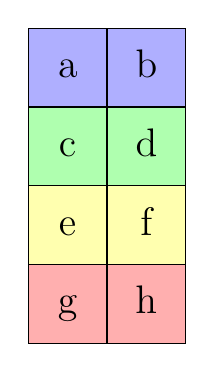
\begin{tikzpicture}[x={(0cm,-1cm)},y={(1cm,0cm)},every node/.style={minimum size=1cm, outer sep=0pt},baseline=(current bounding box.center)]
\node[draw=black, fill={rgb,255:red,175;green,175;blue,255}] at (0,0) {\Large a\strut};
\node[draw=black, fill={rgb,255:red,175;green,175;blue,255}] at (0,1) {\Large b\strut};
\node[draw=black, fill={rgb,255:red,175;green,255;blue,175}] at (1,0) {\Large c\strut};
\node[draw=black, fill={rgb,255:red,175;green,255;blue,175}] at (1,1) {\Large d\strut};
\node[draw=black, fill={rgb,255:red,255;green,255;blue,175}] at (2,0) {\Large e\strut};
\node[draw=black, fill={rgb,255:red,255;green,255;blue,175}] at (2,1) {\Large f\strut};
\node[draw=black, fill={rgb,255:red,255;green,175;blue,175}] at (3,0) {\Large g\strut};
\node[draw=black, fill={rgb,255:red,255;green,175;blue,175}] at (3,1) {\Large h\strut};
\end{tikzpicture}
} &
\shortstack{形状：$(4,2)$\\ 步幅：$(2,1)$} &
\shortstack{形状：$((2,2),2)$\\ 步幅：$((2,4),1)$} \\
\hline
\shortstack{矩阵，$2 {\times} 4$\\ 将模 2 折叠进模 1} &
\scalebox{0.4}{
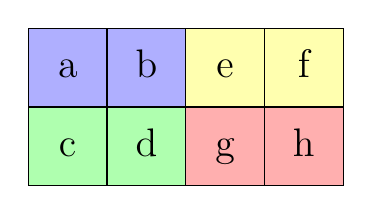
\begin{tikzpicture}[x={(0cm,-1cm)},y={(1cm,0cm)},every node/.style={minimum size=1cm, outer sep=0pt},baseline=(current bounding box.center)]
\node[draw=black, fill={rgb,255:red,175;green,175;blue,255}] at (0,0) {\Large a\strut};
\node[draw=black, fill={rgb,255:red,175;green,175;blue,255}] at (0,1) {\Large b\strut};
\node[draw=black, fill={rgb,255:red,175;green,255;blue,175}] at (1,0) {\Large c\strut};
\node[draw=black, fill={rgb,255:red,175;green,255;blue,175}] at (1,1) {\Large d\strut};
\node[draw=black, fill={rgb,255:red,255;green,255;blue,175}] at (0,2) {\Large e\strut};
\node[draw=black, fill={rgb,255:red,255;green,255;blue,175}] at (0,3) {\Large f\strut};
\node[draw=black, fill={rgb,255:red,255;green,175;blue,175}] at (1,2) {\Large g\strut};
\node[draw=black, fill={rgb,255:red,255;green,175;blue,175}] at (1,3) {\Large h\strut};
\end{tikzpicture}
} &
\shortstack{形状：$(2,4)$\\ 步幅：$(2,\text{\color{red}$\times$})$} &
\shortstack{形状：$(2,(2,2))$\\ 步幅：$(2,(1,4))$} \\
\hline
\end{tabular}
\caption{将一个 8 元素的物理数组视为 3 阶张量，并折叠为两个矩阵。}
\label{fig:folding}
\end{figure}

折叠后矩阵的 \CuTe 表示见最后一列，它强调张量折叠实际上只是把模分组。对 $4 {\times} 2$ 矩阵而言，扁平表示称为 \CuTe 表示的{\em 合并}版本；而对 $2 {\times} 4$ 矩阵，这样的扁平表示并不存在。

这种一般化的张量折叠形式使所有张量收缩都能写成单一的规范收缩形式：
\begin{align}
\mathbf{C}_{\hat{m}\hat{n}\hat{\ell}} = \mathbf{A}_{\hat{m}\hat{k}\hat{\ell}} \, \mathbf{B}_{\hat{n}\hat{k}\hat{\ell}}.
\end{align}
其中每个模可以是单个模，也可以是一组模，我们称之为{\em 多模}（multi-mode）。援引第~\ref{sec:loops} 节的规范化循环：无论 $\hat{m}$ 的形状是 $M$ 还是 $(M_0,M_1)$，我们都可以用 1 维坐标 $m$ 对其循环。于是，任何张量收缩都可以折叠为规范化的 {\tt batched-GEMM}，并用由四重嵌套循环组成的朴素参考实现求值：
\begin{cpp}
for (int l = 0; l < L; ++l)
  for (int m = 0; m < M; ++m)
    for (int n = 0; n < N; ++n)
      for (int k = 0; k < K; ++k)
        C(m,n,l) += A(m,k,l) * B(n,k,l);
\end{cpp}
只要巧妙地构造折叠布局，这个简单的 {\tt batched-GEMM} 实现便可用于求值范围广泛、相互兼容的张量收缩，包括任意矩阵乘法（{\tt GEMM}）、张量收缩（{\tt GETT}）与卷积（{\tt CONV}）。通用 {\tt GEMM} 及其应用的细节见第~\ref{sec:gemm} 节。

随后，优化便可专注于循环重排、分块、向量化这些常见手段，做法都是变换循环嵌套的顺序与阶。这些变换往往可以用布局表示为算法坐标空间上的置换。这些变换布局与数据布局进行函数式复合，生成新的循环嵌套，并保证与原始问题一致。布局复合及其在通用划分中的应用细节见第~\ref{sec:composition} 节。
